\documentclass[11pt, a4paper]{article}

\usepackage[utf8]{inputenc}
\usepackage[T1]{fontenc}
\usepackage[ngerman]{babel}
\usepackage{amsmath}
\usepackage{amssymb}
\usepackage{graphicx}
\usepackage{geometry}
\usepackage{fancyhdr}
\usepackage{enumitem}
\usepackage{array}
\usepackage{eso-pic}

\usepackage{siunitx}
\usepackage[b]{esvect}
\DeclareSIUnit{\litre}{l}
\DeclareSIUnit{\barPr}{bar}

\sisetup{angle-symbol-degree = ^\circ}
\sisetup{locale = DE, separate-uncertainty, inter-unit-product = {},
range-units = brackets, list-units = single, per-mode=symbol-or-fraction}

\makeatletter
\def\input@path{{./}{../../}}
\makeatother
\graphicspath{{./}{../../}}

\geometry{a4paper, top=2.5cm, bottom=2.5cm, left=2.5cm, right=2.5cm}

\input{defs}

\pagestyle{fancy}
\fancyhf{}
\cfoot{\thepage}

\begin{document}
\AddToShipoutPictureBG*{%
  \AtPageUpperLeft{%
    \hspace{2.0cm}%
    \raisebox{-5.cm}{%
      
\includegraphics[width=4cm]{Bilder/Allgemein/LogoFHCampus.png}%
    }%
  }%
}

\begin{center}
    {\Large \textbf{Physikalische Grundlagen}} \\[1em]
    {\large 4. Schriftliche Prüfung: Sommersemester 2026} \\[1em]
    {\large Studiengang: Clinical Engineering}
\end{center}

\vspace{1cm}

\noindent
\begin{tabular}{ll}
    \textbf{Vorname:} & \underline{\hspace{8cm}} \\[0.3cm]
    \textbf{Nachname:} & \underline{\hspace{8cm}} \\
\end{tabular}

\vspace{1cm}

\begin{itemize}[label={$\Diamond$}]
    \item Sie haben 90 min Zeit.
    \item Es sind keine Unterlagen erlaubt.
    \item Sie dürfen einen Taschenrechner verwenden.
    \item Geben Sie klare und verständliche Antworten.
    \item Schreiben Sie leserlich.
    \item Streichen Sie alle bis auf eine Lösung durch.
    \item Jeglicher Versuch unerlaubte Hilfsmittel zu verwenden oder von KommilitonInnen \\
    abzuschreiben, wird mit einer negativen Bewertung des Tests geahndet.
\end{itemize}

\vspace{1cm}

\begin{center}
    \textbf{Viel Erfolg!}
\end{center}

\vspace{2cm}

\begin{flushright}
    \renewcommand{\arraystretch}{1.23}
    \begin{tabular}{l p{2.3cm}}
        \hline
        \noalign{\vskip 0.15cm}
        \textbf{\Large{Punkte:}} & \textbf{\Large{/50}} \\
        \noalign{\vskip 0.1cm}
        \hline
        Beispiel 1: & /13 \\
        Beispiel 2: & /14 \\
        Beispiel 3: & /13 \\
        Beispiel 4: & /10
    \end{tabular}
\end{flushright}

\newpage

\section*{Beispiel 1 - Temperaturmischung}

Ein Aluminiumblock mit der Masse $m_{\text{Al}} = \SI{0.65}{\kilogram}$ hat anfangs die Temperatur $T_{\text{Al}} = \SI{180}{\degreeCelsius}$. Er wird in ein wärmeisoliertes Gefäß mit $V_{\text{W}} = \SI{1.5}{\litre}$ Wasser der Anfangstemperatur $T_{\text{W}} = \SI{20}{\degreeCelsius}$ gelegt.

Gegeben sind:
\begin{itemize}
    \item Spezifische Wärmekapazität von Aluminium: $c_{\text{Al}} = \SI{0.90}{\kilo\joule\per(\kilogram\cdot\kelvin)}$
    \item Spezifische Wärmekapazität von Wasser: $c_{\text{W}} = \SI{4.18}{\kilo\joule\per(\kilogram\cdot\kelvin)}$
    \item Dichte von Wasser: $\rho_{\text{W}} = \SI{1.0}{\kilogram\per\deci\metre\cubed}$
\end{itemize}

\begin{center}
    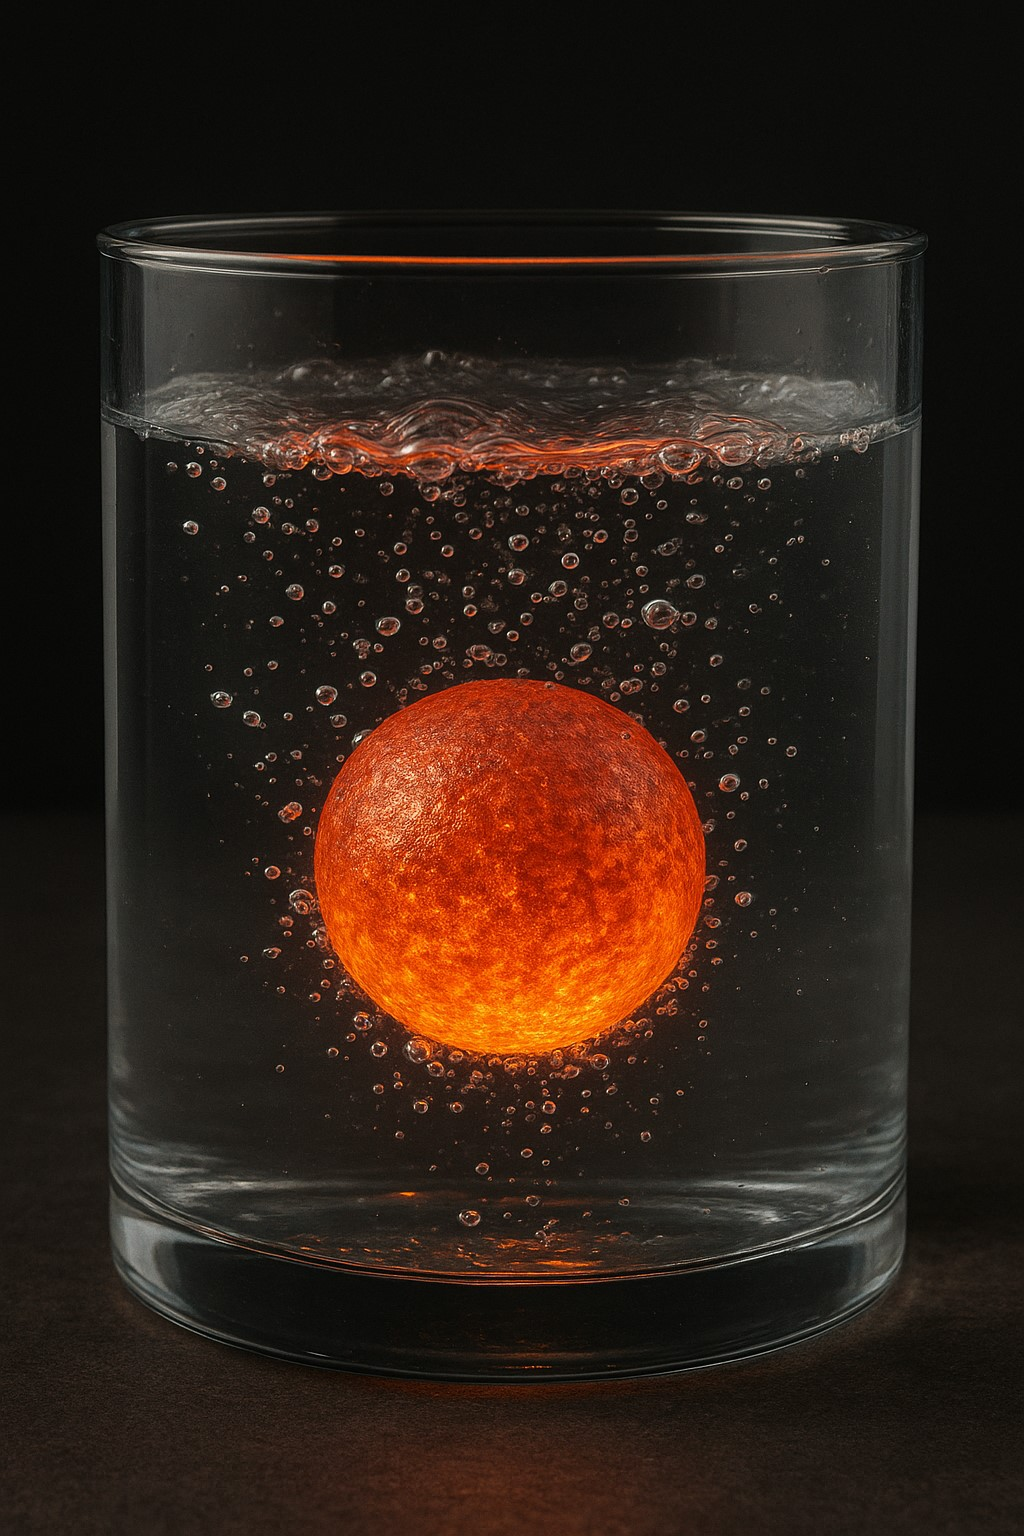
\includegraphics[width=0.3\textwidth]{Bilder/Test/3terAntritt/kugel_in_wasser_3.jpeg}
\end{center}

\subsection*{Aufgabe}
Berechnen Sie die Mischtemperatur $T_{\text{Misch}}$, die sich im thermischen Gleichgewicht einstellt.

\subsection*{Vorgehen}
\begin{enumerate}
    \item Formulieren Sie den Grundsatz des thermischen Gleichgewichts in einem isolierten System. Welche Beziehung besteht zwischen der vom Aluminium abgegebenen und der vom Wasser aufgenommenen Wärme?
    \item Berechnen Sie zunächst die Masse des Wassers.
    \item Stellen Sie eine Formel für die vom Aluminium abgegebene Wärme $Q_{\text{ab}}$ als Funktion von $T_{\text{Misch}}$ auf.
    \item Stellen Sie eine Formel für die vom Wasser aufgenommene Wärme $Q_{\text{auf}}$ als Funktion von $T_{\text{Misch}}$ auf.
    \item Setzen Sie die beiden Wärmeformeln gleich und berechnen Sie die Mischtemperatur $T_{\text{Misch}}$.
\end{enumerate}

\vfill
\begin{flushright}
\renewcommand{\arraystretch}{1.23}
\begin{tabular}{|c | c | c | c | c|}
\hline
\multicolumn{5}{|l|}{\textbf{\large{Punkte: \quad\quad\quad /13}}}\\
\hline
\textbf{1)} & \textbf{2)} & \textbf{3)} & \textbf{4)} & \textbf{5)} \\
\quad/1 & \quad/2 & \quad/2 & \quad/2 & \quad/6 \\
\hline
\end{tabular}
\end{flushright}

\newpage

\section*{Beispiel 2 - Schlittenfahren am Iglu}

Ein Schlittenfahrer der Masse $m$ startet aus der Ruhe am höchsten Punkt ($\alpha = 0$) eines halbkugelförmigen Iglus mit Radius $R$. Gesucht ist der Winkel $\alpha_{\text{max}}$, bei dem der Schlittenfahrer den Kontakt zum Iglu verliert und abhebt. Verwenden Sie das mitgeführte Koordinatensystem $(\ivecS{e}{r}, \ivecS{e}{t})$.

\begin{center}
    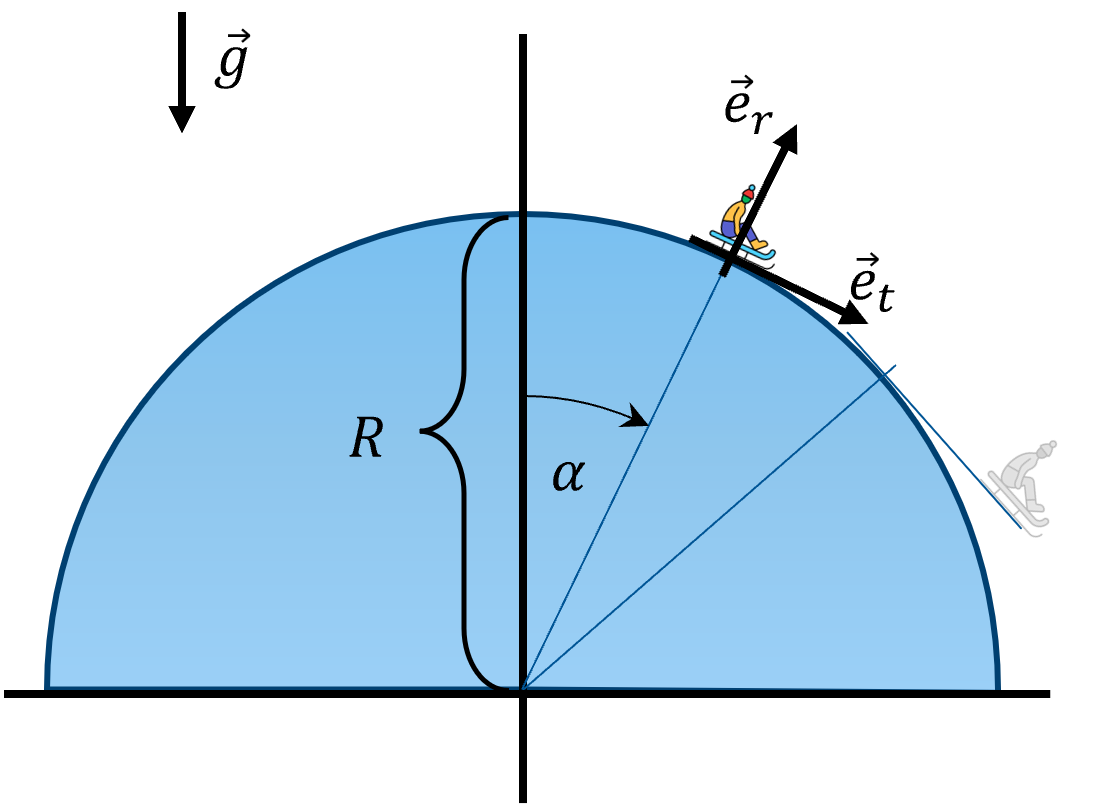
\includegraphics[width=0.50\linewidth]{Bilder/Uebungsaufgaben/schlittenfahren_iglu.png}
\end{center}

\subsection*{Aufgabe}
Leiten Sie mithilfe des zweiten Newtonschen Gesetzes und des Energieerhaltungssatzes den Winkel $\alpha_{\text{max}}$ her, bei dem der Schlittenfahrer vom Iglu abhebt.

\subsection*{Vorgehen}
\begin{enumerate}
    \item Zeichnen Sie die auf den Schlittenfahrer wirkenden Kräfte ($\ivecS{F}{G}$ und $\ivecS{F}{N}$) in die Skizze ein und geben Sie die radialen und tangentialen Komponenten $F_{G,r}$, $F_{G,t}$, $F_{N,r}$ und $F_{N,t}$ an.
    \item Stellen Sie die Bewegungsgleichungen in radialer und tangentialer Richtung mit dem zweiten Newtonschen Gesetz auf.
    \item Im Moment des Abhebens gilt $F_N = 0$. Außerdem ist die Radialbeschleunigung die Zentripetalbeschleunigung $a_r = -v^2/R$. Leiten Sie damit einen Zusammenhang zwischen $v$ und $\alpha_{\text{max}}$ her.
    \item Nutzen Sie den Energieerhaltungssatz, um $v^2$ als Funktion des Winkels $\alpha$ auszudrücken.
    \item Setzen Sie beide Beziehungen zusammen und bestimmen Sie $\alpha_{\text{max}}$. Geben Sie den Winkel auch numerisch in Grad an.
\end{enumerate}

\vfill
\begin{flushright}
\renewcommand{\arraystretch}{1.23}
\begin{tabular}{|c | c | c | c | c|}
\hline
\multicolumn{5}{|l|}{\textbf{\large{Punkte: \quad\quad\quad /14}}}\\
\hline
\textbf{1)} & \textbf{2)} & \textbf{3)} & \textbf{4)} & \textbf{5)} \\
\quad/3 & \quad/3 & \quad/3 & \quad/2.5 & \quad/2.5 \\
\hline
\end{tabular}
\end{flushright}

\newpage

\section*{Beispiel 3 - Ideales Gas im Zylinder}

In einem Zylinder mit beweglichem, reibungsfreiem Kolben befinden sich $n = \SI{1.50}{\mole}$ eines einatomigen idealen Gases. Anfangszustand: $p = \SI{120}{\kilo\pascal}$ und $T_1 = \SI{20}{\degreeCelsius}$. Das Gas wird anschließend bei konstantem Druck auf $T_2 = \SI{140}{\degreeCelsius}$ erwärmt.

Gegeben sind:
\begin{itemize}
    \item Universelle Gaskonstante: $R = \SI{8.314}{\joule\per(\mole\cdot\kelvin)}$
    \item Für ein einatomiges ideales Gas: $C_V = \frac{3}{2}R$ und $C_P = \frac{5}{2}R$
\end{itemize}

\subsection*{Aufgabe}
Berechnen Sie das Anfangsvolumen $V_1$, das Endvolumen $V_2$, die Volumenarbeit $W$, die Änderung der inneren Energie $\Delta U$ und die zugeführte Wärme $Q$.

\subsection*{Vorgehen}
\begin{enumerate}
    \item Rechnen Sie die Temperaturen $T_1$ und $T_2$ in Kelvin um.
    \item Berechnen Sie mit der Zustandsgleichung des idealen Gases das Anfangsvolumen $V_1$.
    \item Welche Beziehung gilt bei einer isobaren Zustandsänderung zwischen Volumen und absoluter Temperatur? Bestimmen Sie damit das Endvolumen $V_2$.
    \item Berechnen Sie die Volumenarbeit $W$ des Gases während der isobaren Erwärmung.
    \item Berechnen Sie die Änderung der inneren Energie $\Delta U$ und daraus mithilfe des 1. Hauptsatzes der Thermodynamik die zugeführte Wärme $Q$.
\end{enumerate}

\vfill
\begin{flushright}
\renewcommand{\arraystretch}{1.23}
\begin{tabular}{|c | c | c | c | c|}
\hline
\multicolumn{5}{|l|}{\textbf{\large{Punkte: \quad\quad\quad /13}}}\\
\hline
\textbf{1)} & \textbf{2)} & \textbf{3)} & \textbf{4)} & \textbf{5)} \\
\quad/2 & \quad/3 & \quad/2 & \quad/3 & \quad/3 \\
\hline
\end{tabular}
\end{flushright}

\newpage

\section*{Beispiel 4 - Single-Choice}
\textit{Kreuzen Sie die korrekte Antwort an. Pro Frage ist nur eine Antwort richtig.}

\begin{enumerate}[label=\arabic*.,itemsep=18pt]
    \item Welche physikalische Größe hat die SI-Einheit \si{\watt}?
    \begin{itemize}[label={$\square$},itemsep=1pt,topsep=0pt]
        \item Arbeit
        \item Energie
        \item Leistung
        \item Kraft
    \end{itemize}

    \item Bei einem isochoren Prozess eines idealen Gases bleibt welche Zustandsgröße konstant?
    \begin{itemize}[label={$\square$},itemsep=1pt,topsep=0pt]
        \item Der Druck
        \item Das Volumen
        \item Die Temperatur
        \item Die innere Energie
    \end{itemize}

    \item Verdoppelt sich die Geschwindigkeit eines Körpers, dann ändert sich seine kinetische Energie um welchen Faktor?
    \begin{itemize}[label={$\square$},itemsep=1pt,topsep=0pt]
        \item Faktor 2
        \item Faktor 4
        \item Faktor 6
        \item Faktor 8
    \end{itemize}

    \item Nach dem archimedischen Prinzip ist die Auftriebskraft gleich ...
    \begin{itemize}[label={$\square$},itemsep=1pt,topsep=0pt]
        \item dem Gewicht des Körpers.
        \item dem Gewicht des verdrängten Mediums.
        \item der Masse des Körpers geteilt durch sein Volumen.
        \item der Gewichtskraft der eingeschlossenen Luft.
    \end{itemize}

    \item Welche Aussage beschreibt das 3. Newtonsche Axiom?
    \begin{itemize}[label={$\square$},itemsep=1pt,topsep=0pt]
        \item Ohne resultierende Kraft bleibt die Geschwindigkeit konstant.
        \item Die Beschleunigung ist proportional zur Kraft.
        \item Kräfte treten paarweise als gleich große, entgegengesetzt gerichtete Wechselwirkungen auf.
        \item Energie kann nicht erzeugt oder vernichtet werden.
    \end{itemize}

    \newpage
    \item Die absolute Temperatur eines idealen Gases ist ein Maß für die ...
    \begin{itemize}[label={$\square$},itemsep=1pt,topsep=0pt]
        \item mittlere potentielle Energie der Teilchen.
        \item mittlere kinetische Energie der Teilchen.
        \item Anzahl der Teilchen.
        \item Dichte des Gases.
    \end{itemize}

    \item Das Produkt $p \cdot V$ hat in der Physik dieselbe Einheit wie welche physikalische Größe?
    \begin{itemize}[label={$\square$},itemsep=1pt,topsep=0pt]
        \item Kraft, Einheit: \si{\newton}
        \item Druck, Einheit: \si{\pascal}
        \item Arbeit, Einheit: \si{\joule}
        \item Impuls, Einheit: \si{\kilogram\cdot \metre\per\second}
        \item Leistung, Einheit: \si{\watt}
    \end{itemize}

    \item Welche Aussage zum idealen Carnot-Prozess ist richtig?
    \begin{itemize}[label={$\square$},itemsep=1pt,topsep=0pt]
        \item Sein Wirkungsgrad hängt nur vom Arbeitsgas ab.
        \item Sein Wirkungsgrad hängt nur von den Temperaturen des heißen und kalten Reservoirs in Kelvin ab.
        \item Er besteht aus zwei isochoren und zwei isobaren Zustandsänderungen.
        \item Sein Wirkungsgrad kann größer als 100\% werden.
    \end{itemize}

    \item Bei konstanter Stoffmenge und konstantem Volumen wird die absolute Temperatur eines idealen Gases verdoppelt. Was geschieht mit dem Druck?
    \begin{itemize}[label={$\square$},itemsep=1pt,topsep=0pt]
        \item Der Druck halbiert sich.
        \item Der Druck bleibt konstant.
        \item Der Druck verdoppelt sich.
        \item Der Druck vervierfacht sich.
    \end{itemize}

    \item Welcher Hauptsatz der Thermodynamik erklärt, warum Wärme nicht spontan von einem kälteren zu einem wärmeren Körper fließt?
    \begin{itemize}[label={$\square$},itemsep=1pt,topsep=0pt]
        \item Der nullte Hauptsatz
        \item Der erste Hauptsatz
        \item Der zweite Hauptsatz
        \item Der dritte Hauptsatz
    \end{itemize}
\end{enumerate}

\vfill
\begin{flushright}
\renewcommand{\arraystretch}{1.23}
\begin{tabular}{|l c|}
\hline
\multicolumn{2}{|l|}{\textbf{\large{Punkte: \quad\quad\quad /10}}}\\
\hline
\textbf{1--10: je /1} & \\
\hline
\end{tabular}
\end{flushright}

\end{document}\documentclass[11pt, a4paper]{article}

\usepackage[utf8]{inputenc}
\usepackage[T1]{fontenc}
\usepackage[ngerman]{babel}
\usepackage{amsmath}
\usepackage{amssymb}
\usepackage{graphicx}
\usepackage{geometry}
\usepackage{fancyhdr}
\usepackage{enumitem}
\usepackage{array}
\usepackage{eso-pic}

\usepackage{siunitx}
\DeclareSIUnit{\litre}{l}
\DeclareSIUnit{\barPr}{bar}

\sisetup{angle-symbol-degree = ^\circ}
\sisetup{locale = DE, separate-uncertainty, inter-unit-product = {},
range-units = brackets, list-units = single, per-mode=symbol-or-fraction}

\makeatletter
\def\input@path{{./}{../../}}
\makeatother
\graphicspath{{./}{../../}}

\geometry{a4paper, top=2.5cm, bottom=2.5cm, left=2.5cm, right=2.5cm}

\input{defs}

\pagestyle{fancy}
\fancyhf{}
\cfoot{\thepage}

\begin{document}
\AddToShipoutPictureBG*{%
  \AtPageUpperLeft{%
    \hspace{2.0cm}%
    \raisebox{-5.cm}{%
      
\includegraphics[width=4cm]{Bilder/Allgemein/LogoFHCampus.png}%
    }%
  }%
}

\begin{center}
    {\Large \textbf{Physikalische Grundlagen}} \\[1em]
    {\large 4. Schriftliche Pr"ufung: Sommersemester 2026} \\[1em]
    {\large Studiengang: Clinical Engineering}
\end{center}

\vspace{1cm}

\noindent
\begin{tabular}{ll}
    \textbf{Vorname:} & \underline{\hspace{8cm}} \\[0.3cm]
    \textbf{Nachname:} & \underline{\hspace{8cm}} \\
\end{tabular}

\vspace{1cm}

\begin{itemize}[label={$\Diamond$}]
    \item Sie haben 90 min Zeit.
    \item Es sind keine Unterlagen erlaubt.
    \item Sie d"urfen einen Taschenrechner verwenden.
    \item Geben Sie klare und verst"andliche Antworten.
    \item Schreiben Sie leserlich.
    \item Streichen Sie alle bis auf eine L"osung durch.
    \item Jeglicher Versuch unerlaubte Hilfsmittel zu verwenden oder von KommilitonInnen \\
    abzuschreiben, wird mit einer negativen Bewertung des Tests geahndet.
\end{itemize}

\vspace{1cm}

\begin{center}
    \textbf{Viel Erfolg!}
\end{center}

\vspace{2cm}

\begin{flushright}
    \renewcommand{\arraystretch}{1.23}
    \begin{tabular}{l p{2.3cm}}
        \hline
        \noalign{\vskip 0.15cm}
        \textbf{\Large{Punkte:}} & \textbf{\Large{/50}} \\
        \noalign{\vskip 0.1cm}
        \hline
        Beispiel 1: & /13 \\
        Beispiel 2: & /14 \\
        Beispiel 3: & /13 \\
        Beispiel 4: & /10
    \end{tabular}
\end{flushright}

\newpage

\section*{Beispiel 1 - Temperaturmischung}

Ein Kupferblock der Masse $m_{\text{Cu}} = \SI{0.60}{\kilogram}$ mit der Anfangstemperatur $T_{\text{Cu}} = \SI{180}{\degreeCelsius}$ wird in ein w"armeisoliertes Gef"a\ss{} mit $V_{\text{W}} = \SI{1.5}{\litre}$ Wasser der Anfangstemperatur $T_{\text{W}} = \SI{18}{\degreeCelsius}$ gelegt. Die W"armekapazit"at des Gef"a\ss es soll vernachl"assigt werden.

Gegeben sind:
\begin{itemize}
    \item Spezifische W"armekapazit"at von Kupfer: $c_{\text{Cu}} = \SI{0.385}{\kilo\joule\per(\kilogram\cdot\kelvin)}$
    \item Spezifische W"armekapazit"at von Wasser: $c_{\text{W}} = \SI{4.18}{\kilo\joule\per(\kilogram\cdot\kelvin)}$
    \item Dichte von Wasser: $\rho_{\text{W}} = \SI{1.0}{\kilogram\per\litre}$
\end{itemize}

\begin{center}
    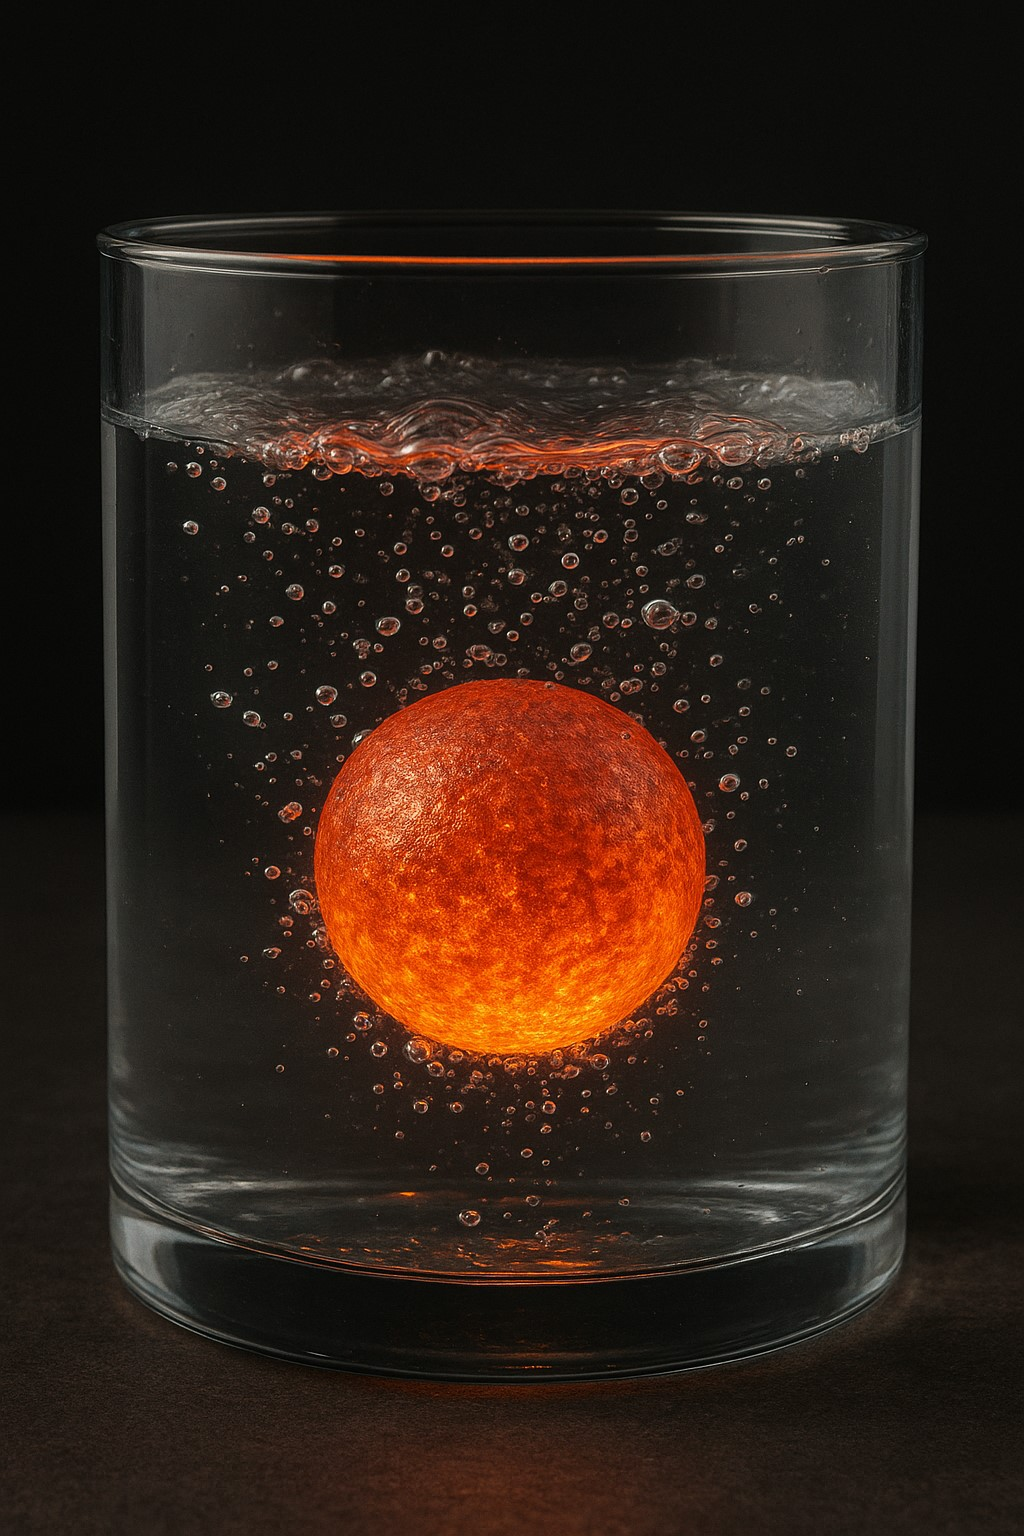
\includegraphics[width=0.28\textwidth]{Bilder/Test/3terAntritt/kugel_in_wasser_3.jpeg}
\end{center}

\subsection*{Aufgabe}
Berechnen Sie die Mischtemperatur $T_{\text{Misch}}$, die sich nach dem thermischen Ausgleich einstellt.

\subsection*{Vorgehen}
\begin{enumerate}
    \item Formulieren Sie den Energieerhaltungssatz f"ur dieses thermisch isolierte System. Welche Beziehung besteht zwischen der vom Kupfer abgegebenen und der vom Wasser aufgenommenen W"arme?
    \item Berechnen Sie aus dem gegebenen Volumen die Masse des Wassers.
    \item Stellen Sie eine Formel f"ur die vom Kupfer abgegebene W"arme $Q_{\text{ab}}$ in Abh"angigkeit von $T_{\text{Misch}}$ auf.
    \item Stellen Sie eine Formel f"ur die vom Wasser aufgenommene W"arme $Q_{\text{auf}}$ in Abh"angigkeit von $T_{\text{Misch}}$ auf.
    \item Bestimmen Sie durch Gleichsetzen von $Q_{\text{ab}}$ und $Q_{\text{auf}}$ die Mischtemperatur $T_{\text{Misch}}$.
\end{enumerate}

\vfill
\begin{flushright}
\renewcommand{\arraystretch}{1.23}
\begin{tabular}{|c | c | c | c | c|}
\hline
\multicolumn{5}{|l|}{\textbf{\large{Punkte: \quad\quad\quad /13}}}\\
\hline
\textbf{1)} & \textbf{2)} & \textbf{3)} & \textbf{4)} & \textbf{5)} \\
\quad/1 & \quad/2 & \quad/2 & \quad/2 & \quad/6 \\
\hline
\end{tabular}
\end{flushright}

\newpage

\section*{Beispiel 2 - Schlittenfahren am Iglu}

Ein Schlittenfahrer der Masse $m$ startet aus der Ruhe am h"ochsten Punkt ($\alpha = 0$) eines halbkugelf"ormigen Iglus mit Radius $R$. Gesucht ist der Winkel $\alpha_{\text{max}}$, bei dem der Schlittenfahrer den Kontakt zum Iglu verliert und abhebt. Verwenden Sie das mitgef"uhrte Koordinatensystem $(\ivecS{e}{r}, \ivecS{e}{t})$.

\begin{center}
    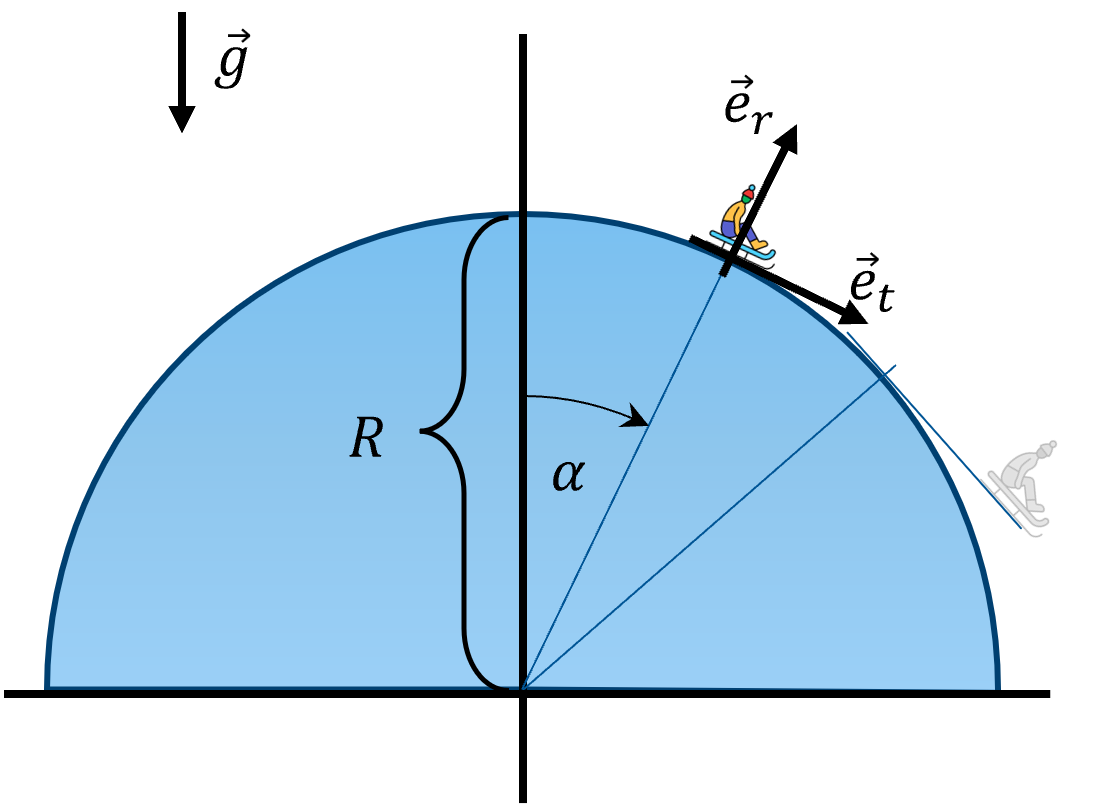
\includegraphics[width=0.50\linewidth]{Bilder/Uebungsaufgaben/schlittenfahren_iglu.png}
\end{center}

\subsection*{Aufgabe}
Leiten Sie den Winkel $\alpha_{\text{max}}$ her, bei dem der Schlittenfahrer den Kontakt zum Iglu verliert.

\subsection*{Vorgehen}
\begin{enumerate}
    \item Zeichnen Sie die auf den Schlittenfahrer wirkenden Kr"afte in die Skizze ein und zerlegen Sie Gewichtskraft und Normalkraft in radiale und tangentiale Komponenten.
    \item Stellen Sie die Bewegungsgleichungen in radialer und tangentialer Richtung mit dem 2. Newtonschen Gesetz auf.
    \item Im Moment des Abhebens gilt $F_N = 0$. Verwenden Sie au\ss{}erdem $a_r = -v^2/R$ und leiten Sie damit einen Zusammenhang zwischen $v$ und $\alpha_{\text{max}}$ her.
    \item Bestimmen Sie mithilfe des Energieerhaltungssatzes die Geschwindigkeit $v$ als Funktion des Winkels $\alpha$.
    \item Setzen Sie beide Beziehungen zusammen und bestimmen Sie $\alpha_{\text{max}}$ in Grad. Geben Sie kurz an, ob das Ergebnis von $m$ oder $R$ abh"angt.
\end{enumerate}

\vfill
\begin{flushright}
\renewcommand{\arraystretch}{1.23}
\begin{tabular}{|c | c | c | c | c|}
\hline
\multicolumn{5}{|l|}{\textbf{\large{Punkte: \quad\quad\quad /14}}}\\
\hline
\textbf{1)} & \textbf{2)} & \textbf{3)} & \textbf{4)} & \textbf{5)} \\
\quad/3 & \quad/3 & \quad/3 & \quad/2.5 & \quad/2.5 \\
\hline
\end{tabular}
\end{flushright}

\newpage

\section*{Beispiel 3 - Ideales Gas im Zylinder}

In einem Zylinder mit reibungsfrei beweglichem Kolben befinden sich $n = \SI{1.5}{\mole}$ eines einatomigen idealen Gases. Anfangs herrschen der Druck $p = \SI{1.20}{\barPr}$ und die Temperatur $T_1 = \SI{20}{\degreeCelsius}$. Das Gas wird anschlie\ss{}end bei konstantem Druck auf $T_2 = \SI{140}{\degreeCelsius}$ erw"armt.

Verwenden Sie:
\begin{itemize}
    \item universelle Gaskonstante: $R = \SI{8.314}{\joule\per(\mole\cdot\kelvin)}$
    \item molare W"armekapazit"at bei konstantem Volumen: $C_V = \frac{3}{2}R$
    \item molare W"armekapazit"at bei konstantem Druck: $C_P = \frac{5}{2}R$
\end{itemize}

\subsection*{Aufgabe}
Berechnen Sie das Anfangsvolumen, das Endvolumen, die vom Gas verrichtete Volumenarbeit sowie die "Anderung der inneren Energie und die zugef"uhrte W"arme.

\subsection*{Vorgehen}
\begin{enumerate}
    \item Rechnen Sie die Temperaturen $T_1$ und $T_2$ in Kelvin um.
    \item Berechnen Sie mit der Zustandsgleichung des idealen Gases das Anfangsvolumen $V_1$.
    \item Bestimmen Sie bei konstantem Druck das Endvolumen $V_2$.
    \item Berechnen Sie die vom Gas verrichtete Volumenarbeit $W_{\text{vol}} = p\,(V_2 - V_1)$.
    \item Berechnen Sie die "Anderung der inneren Energie $\Delta U$ und die zugef"uhrte W"arme $Q$.
\end{enumerate}

\vfill
\begin{flushright}
\renewcommand{\arraystretch}{1.23}
\begin{tabular}{|c | c | c | c | c|}
\hline
\multicolumn{5}{|l|}{\textbf{\large{Punkte: \quad\quad\quad /13}}}\\
\hline
\textbf{1)} & \textbf{2)} & \textbf{3)} & \textbf{4)} & \textbf{5)} \\
\quad/1.5 & \quad/2.5 & \quad/2.5 & \quad/3 & \quad/3.5 \\
\hline
\end{tabular}
\end{flushright}

\newpage

\section*{Beispiel 4 - Single-Choice}
\textit{Kreuzen Sie die korrekte Antwort an. Pro Frage ist nur eine Antwort richtig.}

\begin{enumerate}[label=\arabic*.,itemsep=18pt]
    \item Welche physikalische Gr"o\ss{}e hat die SI-Einheit \si{\watt}?
    \begin{itemize}[label={$\square$},itemsep=1pt,topsep=0pt]
        \item Arbeit
        \item Energie
        \item Leistung
        \item Kraft
    \end{itemize}

    \item Verdoppelt sich die Geschwindigkeit eines K"orpers, dann "andert sich seine kinetische Energie um welchen Faktor?
    \begin{itemize}[label={$\square$},itemsep=1pt,topsep=0pt]
        \item Faktor 2
        \item Faktor 4
        \item Faktor 6
        \item Faktor 8
    \end{itemize}

    \item Nach dem archimedischen Prinzip ist die Auftriebskraft gleich ...
    \begin{itemize}[label={$\square$},itemsep=1pt,topsep=0pt]
        \item dem Gewicht des K"orpers.
        \item dem Gewicht des verdr"angten Mediums.
        \item der Masse des K"orpers geteilt durch sein Volumen.
        \item der Gewichtskraft der eingeschlossenen Luft.
    \end{itemize}

    \item Welche Aussage beschreibt das 3. Newtonsche Axiom?
    \begin{itemize}[label={$\square$},itemsep=1pt,topsep=0pt]
        \item Ohne resultierende Kraft bleibt die Geschwindigkeit konstant.
        \item Die Beschleunigung ist proportional zur Kraft.
        \item Kr"afte treten paarweise als gleich gro\ss{}e, entgegengesetzt gerichtete Wechselwirkungen auf.
        \item Energie kann nicht erzeugt oder vernichtet werden.
    \end{itemize}

    \item Der maximale Wirkungsgrad einer Carnot-Maschine h"angt nur von welchen Gr"o\ss{}en ab?
    \begin{itemize}[label={$\square$},itemsep=1pt,topsep=0pt]
        \item Nur vom Arbeitsgas im Motor
        \item Nur von den Temperaturen des hei\ss{}en und kalten Reservoirs
        \item Nur vom zugef"uhrten Volumen
        \item Nur vom Druck im kalten Reservoir
    \end{itemize}

    \newpage
    \item Ein ideales Gas befindet sich in einem starren Beh"alter. Was geschieht mit dem Druck, wenn sich die absolute Temperatur verdoppelt?
    \begin{itemize}[label={$\square$},itemsep=1pt,topsep=0pt]
        \item Der Druck halbiert sich.
        \item Der Druck bleibt konstant.
        \item Der Druck verdoppelt sich.
        \item Der Druck vervierfacht sich.
    \end{itemize}

    \item Welche Aussage entspricht dem 2. Hauptsatz der Thermodynamik am besten?
    \begin{itemize}[label={$\square$},itemsep=1pt,topsep=0pt]
        \item W"arme flie\ss{}t von selbst immer vom k"alteren zum w"armeren K"orper.
        \item Jede zugef"uhrte W"arme kann vollst"andig in Arbeit umgewandelt werden.
        \item W"arme flie\ss{}t von selbst nicht vom k"alteren zum w"armeren K"orper.
        \item Die innere Energie eines abgeschlossenen Systems ist immer null.
    \end{itemize}

    \item Ein Punkt auf dem Rand einer Scheibe hat den Abstand $r = \SI{0.5}{\metre}$ vom Mittelpunkt. Die Scheibe rotiert mit $\omega = \SI{6}{\radian\per\second}$. Wie gro\ss{} ist die Bahngeschwindigkeit?
    \begin{itemize}[label={$\square$},itemsep=1pt,topsep=0pt]
        \item \SI{3}{\metre\per\second}
        \item \SI{6}{\metre\per\second}
        \item \SI{12}{\metre\per\second}
        \item \SI{0.083}{\metre\per\second}
    \end{itemize}

    \item Der 1. Hauptsatz der Thermodynamik ist eine Formulierung des ...
    \begin{itemize}[label={$\square$},itemsep=1pt,topsep=0pt]
        \item Impulserhaltungssatzes.
        \item Energieerhaltungssatzes.
        \item Massenerhaltungssatzes.
        \item Gravitationsgesetzes.
    \end{itemize}

    \item Bei einem isothermen Prozess eines idealen Gases bleibt welche Zustandsgr"o\ss{}e konstant?
    \begin{itemize}[label={$\square$},itemsep=1pt,topsep=0pt]
        \item Der Druck
        \item Das Volumen
        \item Die Temperatur
        \item Die Stoffmenge
    \end{itemize}
\end{enumerate}

\vfill
\begin{flushright}
\renewcommand{\arraystretch}{1.23}
\begin{tabular}{|l c|}
\hline
\multicolumn{2}{|l|}{\textbf{\large{Punkte: \quad\quad\quad /10}}}\\
\hline
\textbf{1--10: je /1} & \\
\hline
\end{tabular}
\end{flushright}

\end{document}